% 623369a9-2966-4d95-8ebb-bb74259b7289
\documentclass{article}
\usepackage[utf8]{inputenc}
\usepackage{multicol}
\usepackage{listings}
\usepackage{amssymb}
\usepackage{enumitem}
\usepackage{graphicx}
\usepackage{amsthm}
\usepackage{hyperref}
\usepackage[ruled,vlined]{algorithm2e}
\newtheorem{theorem}{Theorem}
\newtheorem{definition}{Definition}

\usepackage{tikz}
\usetikzlibrary{arrows,automata,positioning,decorations.markings}

\SetKwFunction{currencyConverter}{currencyConverter}
\SetKwProg{Fn}{Function}{}{}
\SetKwProg{Proc}{Procedure}{}{}

%=====================================
%			Assignment 5
%==================== =================

\begin{document}

\title{Weekly Assignment 5}
\date{5th October 2017}
\author{Tony Lopar s1013792}
\maketitle

\paragraph{Deadline:} 11th October 2017, 6pm.
\paragraph{Solutions can be found below the exercises}
\paragraph{Collaboration} The graphs in this document are made in collaboration with Carlo Jessurun. We collaborated with creating the graphs in LaTeX. However, we applied our own solutions in the graphs and descriptions.

\section*{Exercise 1. \textit{Weight: 12,5\%}}

Run the Bellman-Ford algorithm on the following directed graph, using vertex $s$ as the source. In each pass, relax edges in the the following order: $(t,x)$, $(t,y)$, $(t,z)$, $(x,t)$, $(y,x)$, $(y,z)$, $(z,x)$, $(z,s)$, $(s,t)$, $(s,y)$. Show the $d$ and $\pi$ values after each pass.


% \begin{center}
	% \includegraphics{img/bellman-ford.pdf}
% \end{center}

\subsection*{Solutions 1}
\begin{enumerate}
    \item The initialization takes place. All values of d are set to infinity, except s which is set to 0, since it's the source. We have 6 vertices which means we will do 5 iterations to decide the shortest path and after these 5 iterations one more iteration to detect any negative weight-cycle.
    \item We start with the first iteration. We will relax the edges in the specified order.
        \begin{enumerate}[label=(\roman*)]
            \item We start by relaxing the from t, since d for t is $\infty$, we can't find a shorter path for any of the edges.
            \item We resume to x. Since d for x is also $\infty$, we can't find a shorter path for any of the edges.
            \item We resume to y. Since d for y is also $\infty$, we can't find a shorter path for any of the edges.
            \item We resume to z. Since d for y is also $\infty$, we can't find a shorter path for any of the edges.
            \item We resume to s. The d for s is 0, so we can define the shortest path for the adjacencies. We will start with the adjacency t, which will become 6. We continue with the adjacency y which will become 7. The $\pi$ of t and y will be s.
            \item We iterated through all edges, so we continue to the second iteration
        \end{enumerate}
    \item We continue with the second iteration. We will relax the edges in the same order as in the first iteration to find possible shorter paths.
        \begin{enumerate}[label=(\roman*)]
            \item We start by relaxing the from t, the sortest path to t is 6. When we iterate through it's adjacencies, we find the following paths to the adjacencies: x = 5, y = 8, z = -4. Since we have already a shorter path for y, we will only modify x and z and assign t as $\pi$ of x and z.
            \item We resume to x. The shortest path to x is 11. From x we only find the adjacency t with an edge of -2. This means the path to t would be 9, but since we already have a shorter path to t, we won't modify it.
            \item We resume to y. The shortest path to y is 7. When we iterate through it's adjacencies, we find the following paths to the adjacencies: x = -3, z = 9. Since z has already a shorter path, we will only modify the path to x and assign y as $\pi$ of x.
            \item We resume to z. The shortest path to z is 2. When we iterate through it's adjacencies, we find the following paths to the adjacencies: x = 7, s = 2. Since x and s both already have a shorter path, we won't modify any of them.
            \item We resume to s. We find adjacencies t and y which have the same shortest path as the current shortest path, so we won't modify them.
            \item We iterated through all edges, so we continue to the third iteration
        \end{enumerate}
    \item We continue with the third iteration. We will relax the edges in the same order as in the previous iterations to find possible shorter paths.
        \begin{enumerate}[label=(\roman*)]
            \item We start by relaxing the from t, the sortest path to t is 6. When we iterate through it's adjacencies, we find the following paths to the adjacencies: x = 5, y = 8, z = -4. Since we already have shorter paths for x and y and the same for z, we won't modify anything.
            \item We resume to x. The shortest path to x is 4. From x we only find the adjacency t with an edge of -2. This means the path to t would be 2 which will be the new shortest path.
            \item We resume to y. The shortest path to y is 7. When we iterate through it's adjacencies, we find the following paths to the adjacencies: x = -3, z = 9. Since z has already a shorter path and x the same path, we won't modify any of them.
            \item We resume to z. The shortest path to z is 2. When we iterate through it's adjacencies, we find the following paths to the adjacencies: x = 7, s = 2. Since x and s both already have a shorter path, we won't modify any of them.
            \item We resume to s. We find adjacencies t and y which have the same shortest path as the current shortest path, so we won't modify them.
            \item We iterated through all edges. Sice no values changed in the last iteration, we may assume that in the following iterations also nothing will change, so we will skip them.
        \end{enumerate}
    \item Since in the third iteration no values changed, the following iterations will be the same as the third iteration.
    \item We should do an iteration to detect if there are negative edge cycles. Since nothing changed in the last iterations, we know that there are no negative edge cycles, so we may skip this iteration too.
\end{enumerate}

The shortest paths after each iteration will be as follows. The $\pi$ of the vertices can be found in between the brackets.
\begin{table}[ht]
\centering
\begin{tabular}{|c||c|c|c|c|c|c|}
\hline
Iteration   & s       & t         & x        & y         & z          \\ \hline\hline
0           & 0       & $\infty$  & $\infty$ & $\infty$  & $\infty$   \\ \hline
1           & 0       & 6 (s)     & $\infty$ & 7 (s)     & $\infty$   \\ \hline
2           & 0       & 6 (s)     & 4 (y)    & 7 (s)     & 2 (t)      \\ \hline
3           & 0       & 2 (x)     & 4 (y)    & 7 (s)     & 2 (t)      \\ \hline
4           & 0       & 2 (x)     & 4 (y)    & 7 (s)     & 2 (t)      \\ \hline
Cycle-detection & 0   & 2 (x)     & 4 (y)    & 7 (s)     & 2 (t)      \\ \hline
\end{tabular}
\end{table}


% \begin{center}
% \begin{tikzpicture}[->,>=stealth',shorten >=1pt,auto,node distance=2cm, every loop/.style={},
%                     thick, ,main node/.style={circle,draw,font=\sffamily\Large\bfseries}]

%   \node[label = {[align=center]left:s \\d = \\ $\pi$ = }][main node] (1) {0};
%   \node[label = {[align=center]above:d = \\ $\pi$ = }][main node] (2) [above right of=1] {$\infty$};
%   \node[label = {[align=center]below:d = \\ $\pi$ = }][main node] (3) [below right of=1] {$\infty$};
%   \node[label = {[align=center]above:d = \\ $\pi$ = }][main node] (4) [right of=2] {$\infty$};
%   \node[label = {[align=center]below:d = \\ $\pi$ = }][main node] (5) [ right of=3] {$\infty$};

%   \path[every node/.style={font=\sffamily\normalsize, text = black }]
%     (1) edge[black] node [above] {6} (2)
%         edge[black] node [below] {7} (3)
%     (2) edge[left, black] node [left] {8} (3)
%         edge[bend left, black] node [above] {5} (4)
%         edge[black] node [left] {-4} (5)
%     (3) edge[left, black] node [right] {-3} (4)
%         edge[left, black] node [below] {9} (5)
%     (4) edge[bend left, black] node [below] {-2} (2)
%     (5) edge[left, black] node [left] {7} (4)
%         edge[left, black] node [right] {2} (1);
% \end{tikzpicture}
% \end{center}

\newpage
\section*{Exercise 2. \textit{Weight: 25\%}}
Shortest path algorithms can be applied in currency trading. We want here to exchange money from one currency to another. The problem here is that all conversions are not possible: given two currencies $A$ and $B$, one can exchange money in currency $A$ to get $B$, but the reverse is not always true. Let us consider a exchange graph $G = (V,E)$ between currencies, giving all possible transactions. The graph is directed (for instance, we can exchange from $A$ to $B$ but not from $B$ to $A$). The exchange function is given by function $c$ such that:
\begin{itemize}
	\item an amount $S$ in currency $A$ costs $S \cdot c(A,B)$ in currency $B$
	\item $c(A,B)$ is defined iff $(A,B)$ is an edge of $G$
	\item $c(A,B) > 0$
\end{itemize}

The exchange graph $G' = (V,E, c)$ is weighted by the exchange function. Let $a_1, a_2, \ldots, a_n$ be various currencies (for instance $a_1$ might be dollars, $a_2$ pounds, and $a_3$ euros). An exchange sequence $a_1, a_2, \ldots, a_k$ is the conversion of money in currency $a_1$ to $a_k$ through intermediate currencies $a_2 \ldots a_{k-1}$
\begin{enumerate}
	\item What is the exchange rate from $a_1$ to $a_k$ in the exchange sequence $a_1, a_2, \ldots, a_k$?
	\item In which condition (consider here $G'$) someone can become infinitely rich by exchanging money?
	\item Given 2 exchange sequences $S_1$ and $S_2$, the best one is the one with the highest rate. Suppose now that we know a sequence $S_1$ to exchange currency $A$ in currency $B$, and $S_2$ to exchange currency $A$ in currency $C$. Suppose now that there exists an edge $(C,B)$ in $G$. Write the relaxation condition comparing the sequence rates $S_1$, and $S_2$ then $(C,B)$. Keep the best one.
	\item Write an improved version of the Bellman-Ford algorithm, using this modified relaxation condition, and give the best exchange rates from currency $A$ to all others. Why is that correct?
    % \item Do the same with Dijkstra's algorithm.
\end{enumerate}

\subsection*{Solutions 2}

\begin{enumerate}
    \item $c(a_1, a_2) \cdot c(a_2, a_3) \cdot \dots \cdot c(a_{k - 1}, a_k)$
    \item Someone can become infinitely rich, by finding a cycle between two currencies where the amount of currency A converted from another currency is higher than the initial amount of currency A. By using this cycle to convert money multiple times, someone will get more money after each iteration in the cycle. This higher amount can be converted again through the same cycle, which will give a higher amount of A again.
    \item The relaxation condition should check which exchange will result in a higher amount in B. So, we will first have to compare $S_1$ and $S_2 \cdot w(C, B)$ where $w(C, B)$ is the conversion rate between C and B. If $S_1 \geq S_2 \cdot w(C, B)$, then $S_1$ will give the best conversion. Otherwise we found a more profitable exchange rate for B by first converting to C and then to B.
    \item This algorithm will have a graph and a currency s as input for which we will calculate the rates.
    \begin{algorithm}[ht]
  \DontPrintSemicolon

    \Proc{ \currencyConverter{G, s}}{
    $d[s] \leftarrow 0$ \;
    $\pi[s] = nil$ \;
    \tcp*{Assuming that exchanging a currency with itself will give the same amount, so the rate will be 1}
    $highestRate[s] \leftarrow 1$ \;

    \ForEach{$v \in |V| - {s}$}{
        $d[s] \leftarrow \infty$ \;
        $highestRate[s] \leftarrow \infty$ \;
    }

    \ForEach{$i \leftarrow 1 \KwTo |V| - 1$}{
        \ForEach{$(u, v) \in E$}{
            \If{$d[v] < d[u] \cdot w(u, v)$}{
                $d[v] \leftarrow d[u] \cdot w(u, v)$ \;
                $\pi[v] \leftarrow u$ \;
                $highestRate[v] \leftarrow highestRate[u] \cdot w(u, v)$ \;
            }
        }
    }

    % \ForEach{$(u, v) \in E$}{
    %     \If{$d[v] < d[u] \cdot w(u, v)$}{
    %         \KwRet{Cycle exists!}
    %     }
    % }
    \KwRet{$highestRate$}

  }


    \caption{Best currency conversions}
\end{algorithm}
\end{enumerate}

\newpage

\section*{Exercise 3.  \textit{Weight: 12,5\%}}

Run the Ford-Fulkerson algorithm on the following flow network. For each iteration, pick the shortest augmenting path from $s$ to $t$ and give the residual network. Finally, give the value of the maximum flow and a minimum cut $(S,T)$.

% \begin{center}
	% \includegraphics[scale=0.6]{img/flow.pdf}
% \end{center}

\subsection*{Solutions 3}
For the first iteration we will pick the shortest path from s to t. This is the path s-x-t which has a maximum capacity of 5, so we flow 5 through it. The value of t increases to 5.
\begin{figure}[h]
\begin{center}
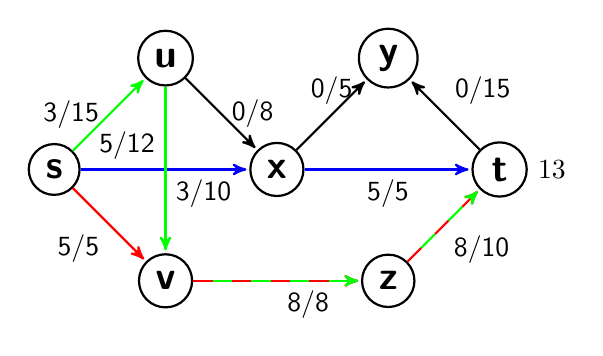
\begin{tikzpicture}[->,>=stealth',shorten >=1pt,auto,node distance=2cm, every loop/.style={},
                    thick, ,main node/.style={circle,draw,font=\sffamily\Large\bfseries}]

  \node[main node] (1) {s};
  \node[main node] (2) [above right of=1] {u};
  \node[main node] (3) [below right of=1] {v};
  \node[main node] (4) [below right of=2] {x};
  \node[main node] (5) [above right of=4] {y};
  \node[main node][label = {[align=center]right:13}] (7) [below right of=5] {t};
  \node[main node] (6) [below left of=7] {z};

  \path[every node/.style={font=\sffamily\normalsize, text = black }]
    (1) edge[green] node [left] {3/15} (2)
        edge[red] node [below left] {5/5} (3)
        edge[blue] node [above left] {5/12} (4)
    (2) edge[black] node [right] {0/8} (4)
        edge[green] node [below right] {3/10} (3)
    (3) edge[red,dash pattern= on 7pt off 7pt] node [below right] {8/8} (6)
        edge[green,dash pattern= on 7pt off 7pt, dash phase=7pt] node [below right] {} (6)
    (4) edge[black] node [above] {0/5} (5)
        edge[blue] node [below] {5/5} (7)
    (6) edge[red,dash pattern= on 7pt off 7pt] node [below right] {8/10} (7)
        edge[green,dash pattern= on 7pt off 7pt, dash phase=7pt] node [below right] {} (7)
    (7) edge[black] node [above right] {0/15} (5);
\end{tikzpicture}
\caption{Max flow} \label{fig:M1}
\end{center}
\end{figure}
\\
From s we try to explore another flow and we find s-v-z-t which has a maximum capacity of 5. The flow to t increases to 10. From v-z-t we can increase the flow three more. We can get this three from s-u-v. Which increases the value of t to 13. A visual representation of the augmented paths can be seen in figure~\ref{fig:M1} where each path is coloured different. From this method I got the maximum flow of 13.

The minimum cut can be found by taking the cut of (x, y), (x, t) and (v, z) which is 18. The edges in this cut are coloured red in figure~\ref{fig:M2}

\begin{figure}[h]
\begin{center}
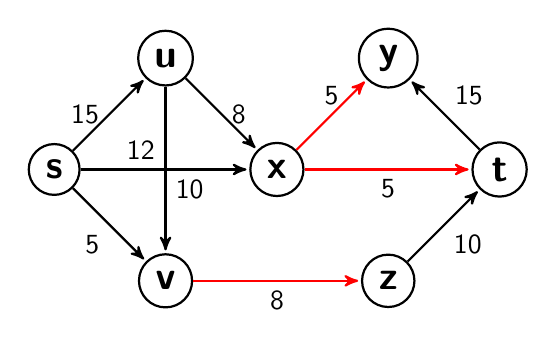
\begin{tikzpicture}[->,>=stealth',shorten >=1pt,auto,node distance=2cm, every loop/.style={},
                    thick, ,main node/.style={circle,draw,font=\sffamily\Large\bfseries}]

  \node[main node] (1) {s};
  \node[main node] (2) [above right of=1] {u};
  \node[main node] (3) [below right of=1] {v};
  \node[main node] (4) [below right of=2] {x};
  \node[main node] (5) [above right of=4] {y};
  \node[main node] (7) [below right of=5] {t};
  \node[main node] (6) [below left of=7] {z};

  \path[every node/.style={font=\sffamily\normalsize, text = black }]
    (1) edge[black] node [left] {15} (2)
        edge[black] node [below left] {5} (3)
        edge[black] node [above left] {12} (4)
    (2) edge[black] node [right] {8} (4)
        edge[black] node [below right] {10} (3)
    (3) edge[left, red] node [below] {8} (6)
    (4) edge[red] node [above] {5} (5)
        edge[red] node [below] {5} (7)
    (6) edge[black] node [below right] {10} (7)
    (7) edge[black] node [above right] {15} (5);
\end{tikzpicture}
\caption{Min cut} \label{fig:M2}
\end{center}
\end{figure}


\newpage


\section*{Exercise 4 . \textit{Weight: 25\%}}
A server $S$ is connected to a computer $T$ via a network composed of nodes $A$, $B$, $C$ and $D$. The transfer capacities (in Mbit/s) are the following:

% \begin{figure}[h!]
% \vspace*{-0.3cm}
% \centering
% \includegraphics[width=3.6cm]{img/ff-1.PNG}
% \vspace*{-0.3cm}
% \end{figure}
The user of machine $T$ downloads a very big file from server $S$. We want to find the routing that maximizes the bit rate.

\begin{enumerate}
  \item Which algorithmic problem does this problem corresponds to? Which algorithm may we use?
  \item Run the algorithm.
  \item What is the maximal bit rate? Which routing enables it?
\end{enumerate}

\subsection*{Solutions 4}
\begin{enumerate}
    \item This situation corresponds to the network flow algorithm, because we want to know how we can get biggest flow which correspondents with the fastest downloadspeed.
    \item First we will represent the flow in a graph. We will take the values from the table as weights of edges. The graph can be found in figure~\ref{fig:M3}  \\
\begin{figure}[h]
    \centering
    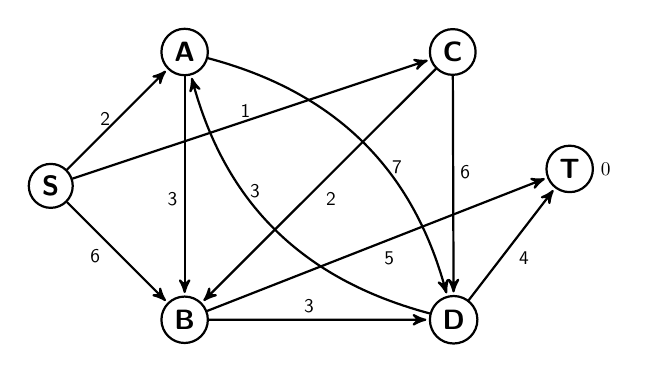
\begin{tikzpicture}[scale=0.7,->,>=stealth',shorten >=1pt,auto,node distance=3cm, every loop/.style={},
                                            thick, ,main node/.style={circle,draw,font=\sffamily\Large\bfseries}, transform shape]

        \node[main node] (1) {S};
        \node[main node] (2) [above right=3cm ] {A};
        \node[main node] (3) [below right=3cm ] {B};
        \node[main node] (5) [right=1cm and 4cm of 2] {C};
        \node[main node] (6) [right=1cm and 4cm of 3] {D};
        \node[main node][label = {[align=center]right:0}] (7) [below right of=5] {T};

        \path[every node/.style={font=\sffamily\normalsize, text = black}, transform shape]
            (1) edge[black] node [left] {2} (2)
                edge[black] node [below left, pos=0.40] {6} (3)
                edge[black] node [above right, pos=0.45] {1} (5)
            (2) edge[bend left, black] node [right, pos=0.60] {7} (6)
                edge[black] node [below left] {3} (3)
            (3) edge[left, black] node [above right, pos=0.40] {3} (6)
                edge[left, black] node [below right] {5} (7)
            (5) edge[left, black] node [below right] {2} (3)
                edge[left, black] node [above right] {6} (6)
            (6) edge[black] node [below right] {4} (7)
                edge[bend left, black] node [right, pos=0.65] {3} (2);
    \end{tikzpicture}
    \caption{Flow network of the situation} \label{fig:M3}
    \end{figure}
    \newline
     The result of the algorithm can be found in figure~\ref{fig:M4}. The augmented paths are marked in different colors to make them clear. Edges where two paths are partially combined are dashed in the figure, these are the edges B-T and D-T.
     \newline
    \begin{figure}[ht]
    \centering
    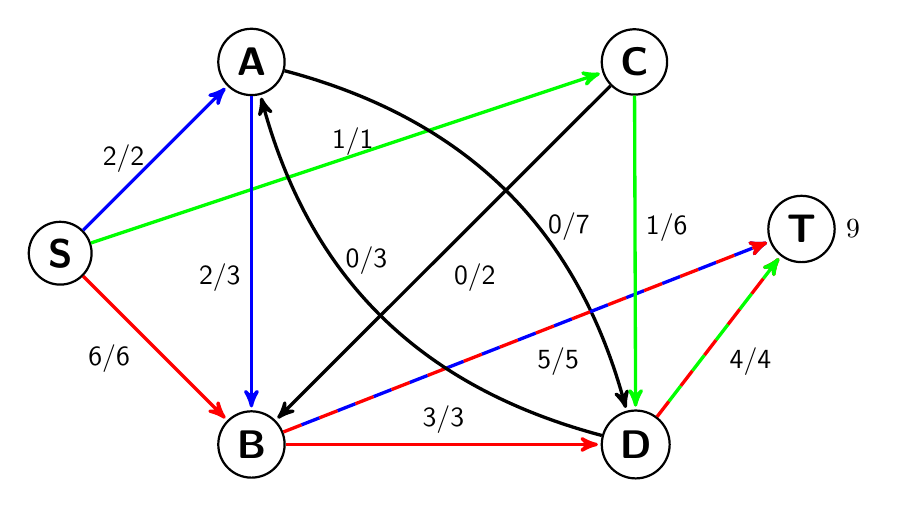
\begin{tikzpicture}[->,>=stealth',shorten >=1pt,auto,node distance=3cm, every loop/.style={}, thick, ,main node/.style={circle,draw,font=\sffamily\Large\bfseries}]

        \node[main node] (1) {S};
        \node[main node] (2) [above right=3cm ] {A};
        \node[main node] (3) [below right=3cm ] {B};
        \node[main node] (5) [right=1cm and 4cm of 2] {C};
        \node[main node] (6) [right=1cm and 4cm of 3] {D};
        \node[main node][label = {[align=center]right:9}] (7) [below right of=5] {T};

        \path[every node/.style={font=\sffamily\normalsize, text = black}, line width=1.2pt]
            (1) edge[blue] node [left] {2/2} (2)
                edge[red] node [below left, pos=0.40] {6/6} (3)
                edge[green] node [above right, pos=0.45] {1/1} (5)
            (2) edge[bend left, black] node [right, pos=0.60] {0/7} (6)
                edge[blue] node [below left] {2/3} (3)
            (3) edge[red] node [above right, pos=0.40] {3/3} (6)
                edge[left, blue,dash pattern= on 7pt off 7pt, dash phase=7pt] node [below right] {5/5} (7)
                edge[left, red,dash pattern= on 7pt off 7pt] node [below right] {} (7)
            (5) edge[left, black] node [below right] {0/2} (3)
                edge[left, green] node [above right] {1/6} (6)
            (6) edge[red,dash pattern= on 7pt off 7pt] node [below right] {4/4} (7)
                edge[green,dash pattern= on 7pt off 7pt, dash phase=7pt] node [below right] {} (7)
                edge[bend left, black] node [right, pos=0.65] {0/3} (2);
    \end{tikzpicture}
    \caption{Flow network after running the algorithm} \label{fig:M4}
    \end{figure}

    \item The maximum bitrate is 9. The routing for this is represented by the coloured edges in figure~\ref{fig:M4}.
\end{enumerate}

\newpage
\section*{Exercise 5. \textit{Weight: 25\%}}

\paragraph{}
A couple wants to organize their wedding dinner.
In order to increase social interactions, they do not want to place two friends or members of a same family at the same table.

Is this possible to model this problem as a maximum flow problem? How?

We consider that there are $p$ disjoint groups of friends/families, the $i$-th group contains $a[i]$ members.
There are also $q$ tables and $b[j]$ seats at the $j$-th table.

\subsection*{Solutions 5}
It is possible to model this with a network flow. The solution I tought of was to create network flow with nodes for all p groups and for all q tables. The capacity to each group from the start is a[i], since this is the number of members in this group. From every group there are flows to every table with a capacity of 1, since from every group only one member may sit at the same table. From every table there will go a flow with capacity b[j] to the sink, because this is the maximum of people that can sit at a table. An example of the solution with two groups and two tables can be seen in figure~\ref{fig:M5}. In this example we have the groups $P_1$ and $P_2$ and the tables $Q_1$ and $Q_2$.

In order to see whether this problem can be solved, we can calculate the max flow of this problem. If the max flow equals the number of guests, then it's possible to have not two members of the same group at the same table. If the max flow is lower, then there must be a group from which all members can't be placed on different tables.

So, this means we can solve this problem using a network flow. A condition is that there is no group with more members than tables, because then it's useless to calculate the max flow, since we already know in advance that not all the members of this group can be placed at a different tables.

\begin{figure}[hb]
    \centering
    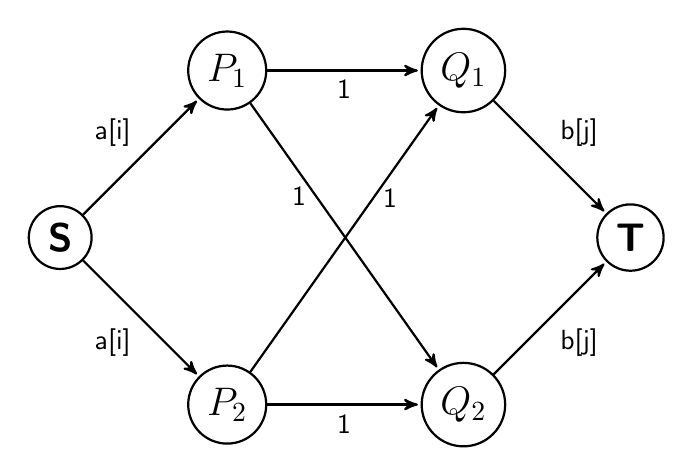
\begin{tikzpicture}[->,>=stealth',shorten >=1pt,auto,node distance=3cm, every loop/.style={},
                                            thick, ,main node/.style={circle,draw,font=\sffamily\Large\bfseries}]

        \node[main node] (1) {S};
        \node[main node] (2) [above right of=1 ] {$P_1$};
        \node[main node] (3) [below right of=1 ] {$P_2$};
        \node[main node] (4) [right of=2] {$Q_1$};
        \node[main node] (5) [right of=3] {$Q_2$};
        \node[main node] (6) [below right of=4] {T};

        \path[every node/.style={font=\sffamily\normalsize, text = black }]
            (1) edge[black] node [above left] {a[i]} (2)
                edge[black] node [below left] {a[i]} (3)
            (2) edge[black] node [below] {1} (4)
                edge[black] node [left, pos=0.35] {1} (5)
            (3) edge[black] node [right, pos=0.65] {1} (4)
                edge[black] node [below] {1} (5)
            (4) edge[black] node [above right] {b[j]} (6)
            (5) edge[black] node [below right] {b[j]} (6);
    \end{tikzpicture}
    \caption{Possible flow network for the wedding problem} \label{fig:M5}
\end{figure}
\end{document}
